\section{Repeated Keys: Completion, Counters and Space}
\label{sec:skew}
The skewed stream contains 67M operations but only \NumDistinctLarge{} distinct keys. Its most frequent key occurs \MaxFrequencyLarge{} times. This distinction changes the task: a set-membership filter can represent each distinct member once, while a counting filter must also preserve the multiplicities through deletion.

\begin{table}[!htbp]\centering\small
\caption{New 67M skewed results at nominal target $1/512$. Rates are means $\pm$ sample SD in M/s. Static filters represent $D$ members and answer the original $N$ positive queries. ``Failed'' refers to incomplete construction; the accepted Cuckoo prefix is reported separately.}
\label{tab:zipf-large}
\begin{tabular}{@{}lrrrrr@{}}
\toprule
\textbf{Filter} & \textbf{Insert} & \textbf{Positive} & \textbf{Negative} & \textbf{Delete} & \textbf{MB} \\
\midrule
CQF & 4.31 $\pm$ 0.05 & 29.06 $\pm$ 2.17 & 18.21 $\pm$ 3.78 & 2.30 $\pm$ 0.15 & 186.808 \\
Cuckoo & Failed & Failed & Failed & Failed & 201.327 \\
Bloom & 74.58 $\pm$ 26.11 & 72.34 $\pm$ 12.43 & 44.39 $\pm$ 3.89 & \na & 0.372 \\
Counting Bloom & 12.16 $\pm$ 0.67 & 15.24 $\pm$ 0.66 & 30.14 $\pm$ 6.68 & 11.65 $\pm$ 1.49 & 9.235 \\
Blocked Bloom & 65.93 $\pm$ 3.60 & 48.77 $\pm$ 2.13 & 50.41 $\pm$ 3.56 & \na & 0.446 \\
XOR & \na & 101.84 $\pm$ 6.19 & 89.80 $\pm$ 2.03 & \na & 0.317 \\
Fuse-style & \na & 102.12 $\pm$ 5.15 & 85.95 $\pm$ 10.35 & \na & 0.333 \\
\bottomrule
\end{tabular}

\end{table}

Cuckoo accepts 24 of 67M insertion operations, a fraction of roughly $3.6\times10^{-7}$. The fixed stream quickly repeats the same key more often than the bucket pair can accommodate. We retain this outcome as a capability result and suppress its partial-run speed and FPR. It does not imply that deduplicating before a set-only Cuckoo build would fail; that would be a different experiment and would not preserve repeated-copy counts.

CQF and Counting Bloom both complete the full stream and all one-occurrence deletions. Bloom and Blocked Bloom also consume every insertion, but offer set membership without deletion. CQF's skewed insertion rate is \CqfInsertSkewLarge{}\Mops{}, compared with \CqfInsertUniformLarge{}\Mops{} on uniform data. Concentrated accesses and counter reuse are consistent with the improvement; we have not measured cache misses or isolated their individual effects.

\begin{figure}[!htbp]\centering
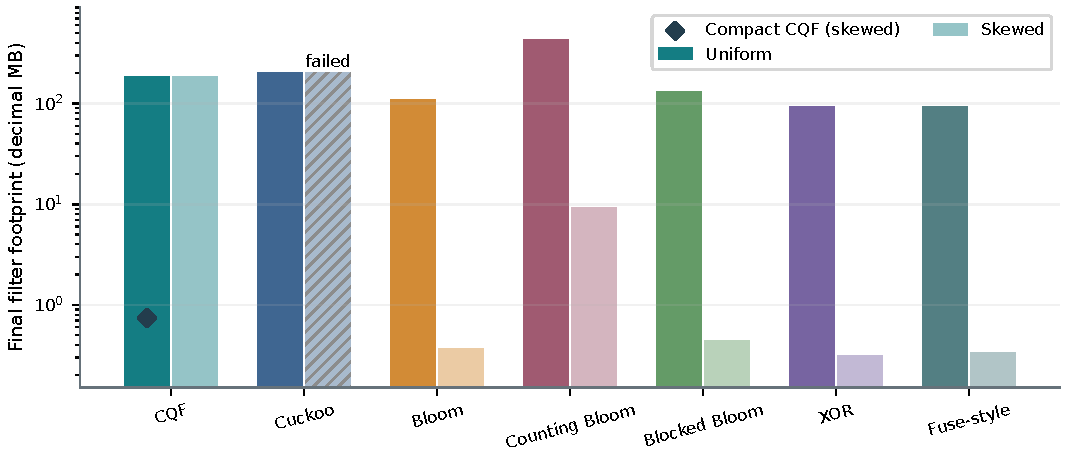
\includegraphics[width=\linewidth]{skew_space.pdf}
\caption{Final footprints under uniform and skewed input at 67M operations. The logarithmic scale keeps small distinct-set structures visible. Cuckoo's failed skewed allocation is marked explicitly. The extra CQF point is a separately sized, one-run sensitivity result; its FPR differs from the primary CQF.}
\label{fig:skew-space}
\end{figure}

The primary CQF reserves \PrimaryCqfMemory{}\,MB from $N$ even though only \SkewOccupiedLarge{} slots are occupied after insertion. By contrast, the Bloom family and immutable filters are allocated from $D$. We therefore also test a separate $2^{19}$-slot CQF at $r=9$ on the same complete skewed stream. It accepts and deletes all 67M occurrences using \CompactMemory{}\,MB. Its measured FPR is \CompactFpr{}, against the $D/2^{28}$ estimate of \CompactExpectedFpr{}. This is a valid target-satisfying operating point in this sample, with less spare capacity and a higher FPR than the primary CQF. Counting Bloom's reported footprint is \CompactCbfMemoryRatio{} times that of this compact CQF, with different achieved accuracy and update rates. This sensitivity point is not a general automatic-sizing algorithm or a proof of minimum capacity.
\finding{Counter compression and allocation policy are separate. A fixed operation-sized CQF can hide the space benefit of counting; a documented capacity sensitivity exposes it without changing the primary comparison.}
\clearpage
